\section{Généralités}

\subsection{Restriction du modèle}

La figure~\ref{modele_restreint} met en évidence le sous ensemble que nous avons choisi d'étudier, qui a été déterminé à partir des contraintes énumérées au chapitre~\ref{chapter:les_contraintes}. Cette sous partie correspond à ce que Laborit nomme le néocortex.

\begin{figure}[H] 
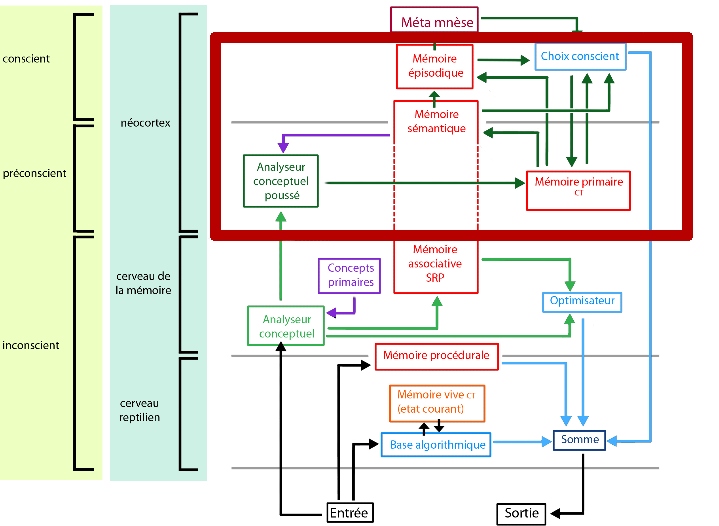
\includegraphics[width=\textwidth]{files/modele_restreint} 
\caption{Modèle restreint déterminé à partir des contraintes énumérée au chapitre~\ref{chapter:les_contraintes}} 
\label{modele_restreint}
\end{figure}

\subsection{Architecture générale}

L'architecture générale de notre modèle est présenté sur la figure ~\ref{schema_general}. L'IA est composé de trois modules :
\begin{itemize}
\item l'analyseur, composé d'un \emph{RuleBook}, d'un analyseur conceptuel de base et d'un analyseur conceptuel poussé,
\item le raisonneur, qui contient un moteur de choix, et un module d'introspection,
\item et la mémoire, structurée avec une interface nommée mémoire primaire.
\end{itemize}
L'environnement est externe à l'agent, et interagit avec ce dernier via ses entées~/~sorties.

Trois niveaux de données sont manipulés par l'IA :
\begin{itemize}
\item les informations basiques, sous la forme de matrices, provenant de l'environnement,
\item un premier niveau correspondant aux concepts primaires,
\item ainsi que les concepts poussés, qui sont stockés en mémoire et qui permettent de raisonner.
\end{itemize}

\subsection{Déroulement d'un coup}

Sur ce schéma, nous pouvons voir que le plateau entre dans notre IA sous forme matricielle. Dans une première étape le \og rule book \fg{} génère un ensemble de plateau à partir des coups possibles. Cette ensemble est fourni à l'analyseur conceptuel de base qui le traduit dans un formalisme logique puis l'analyseur conceptuel poussé associe à chaque plateau un ensemble de formes reconnaissables sur ces plateaux. Le tout est ensuite transmis à la mémoire et le raisonneur et stimulé afin de déclencher la prise de décision. Celui-ci, le raisonneur, effectue une comparaison des plateaux possibles à partir des formes reconnues et une fois sa décision prise la retourne à l'environnement.

\begin{figure}[H] 
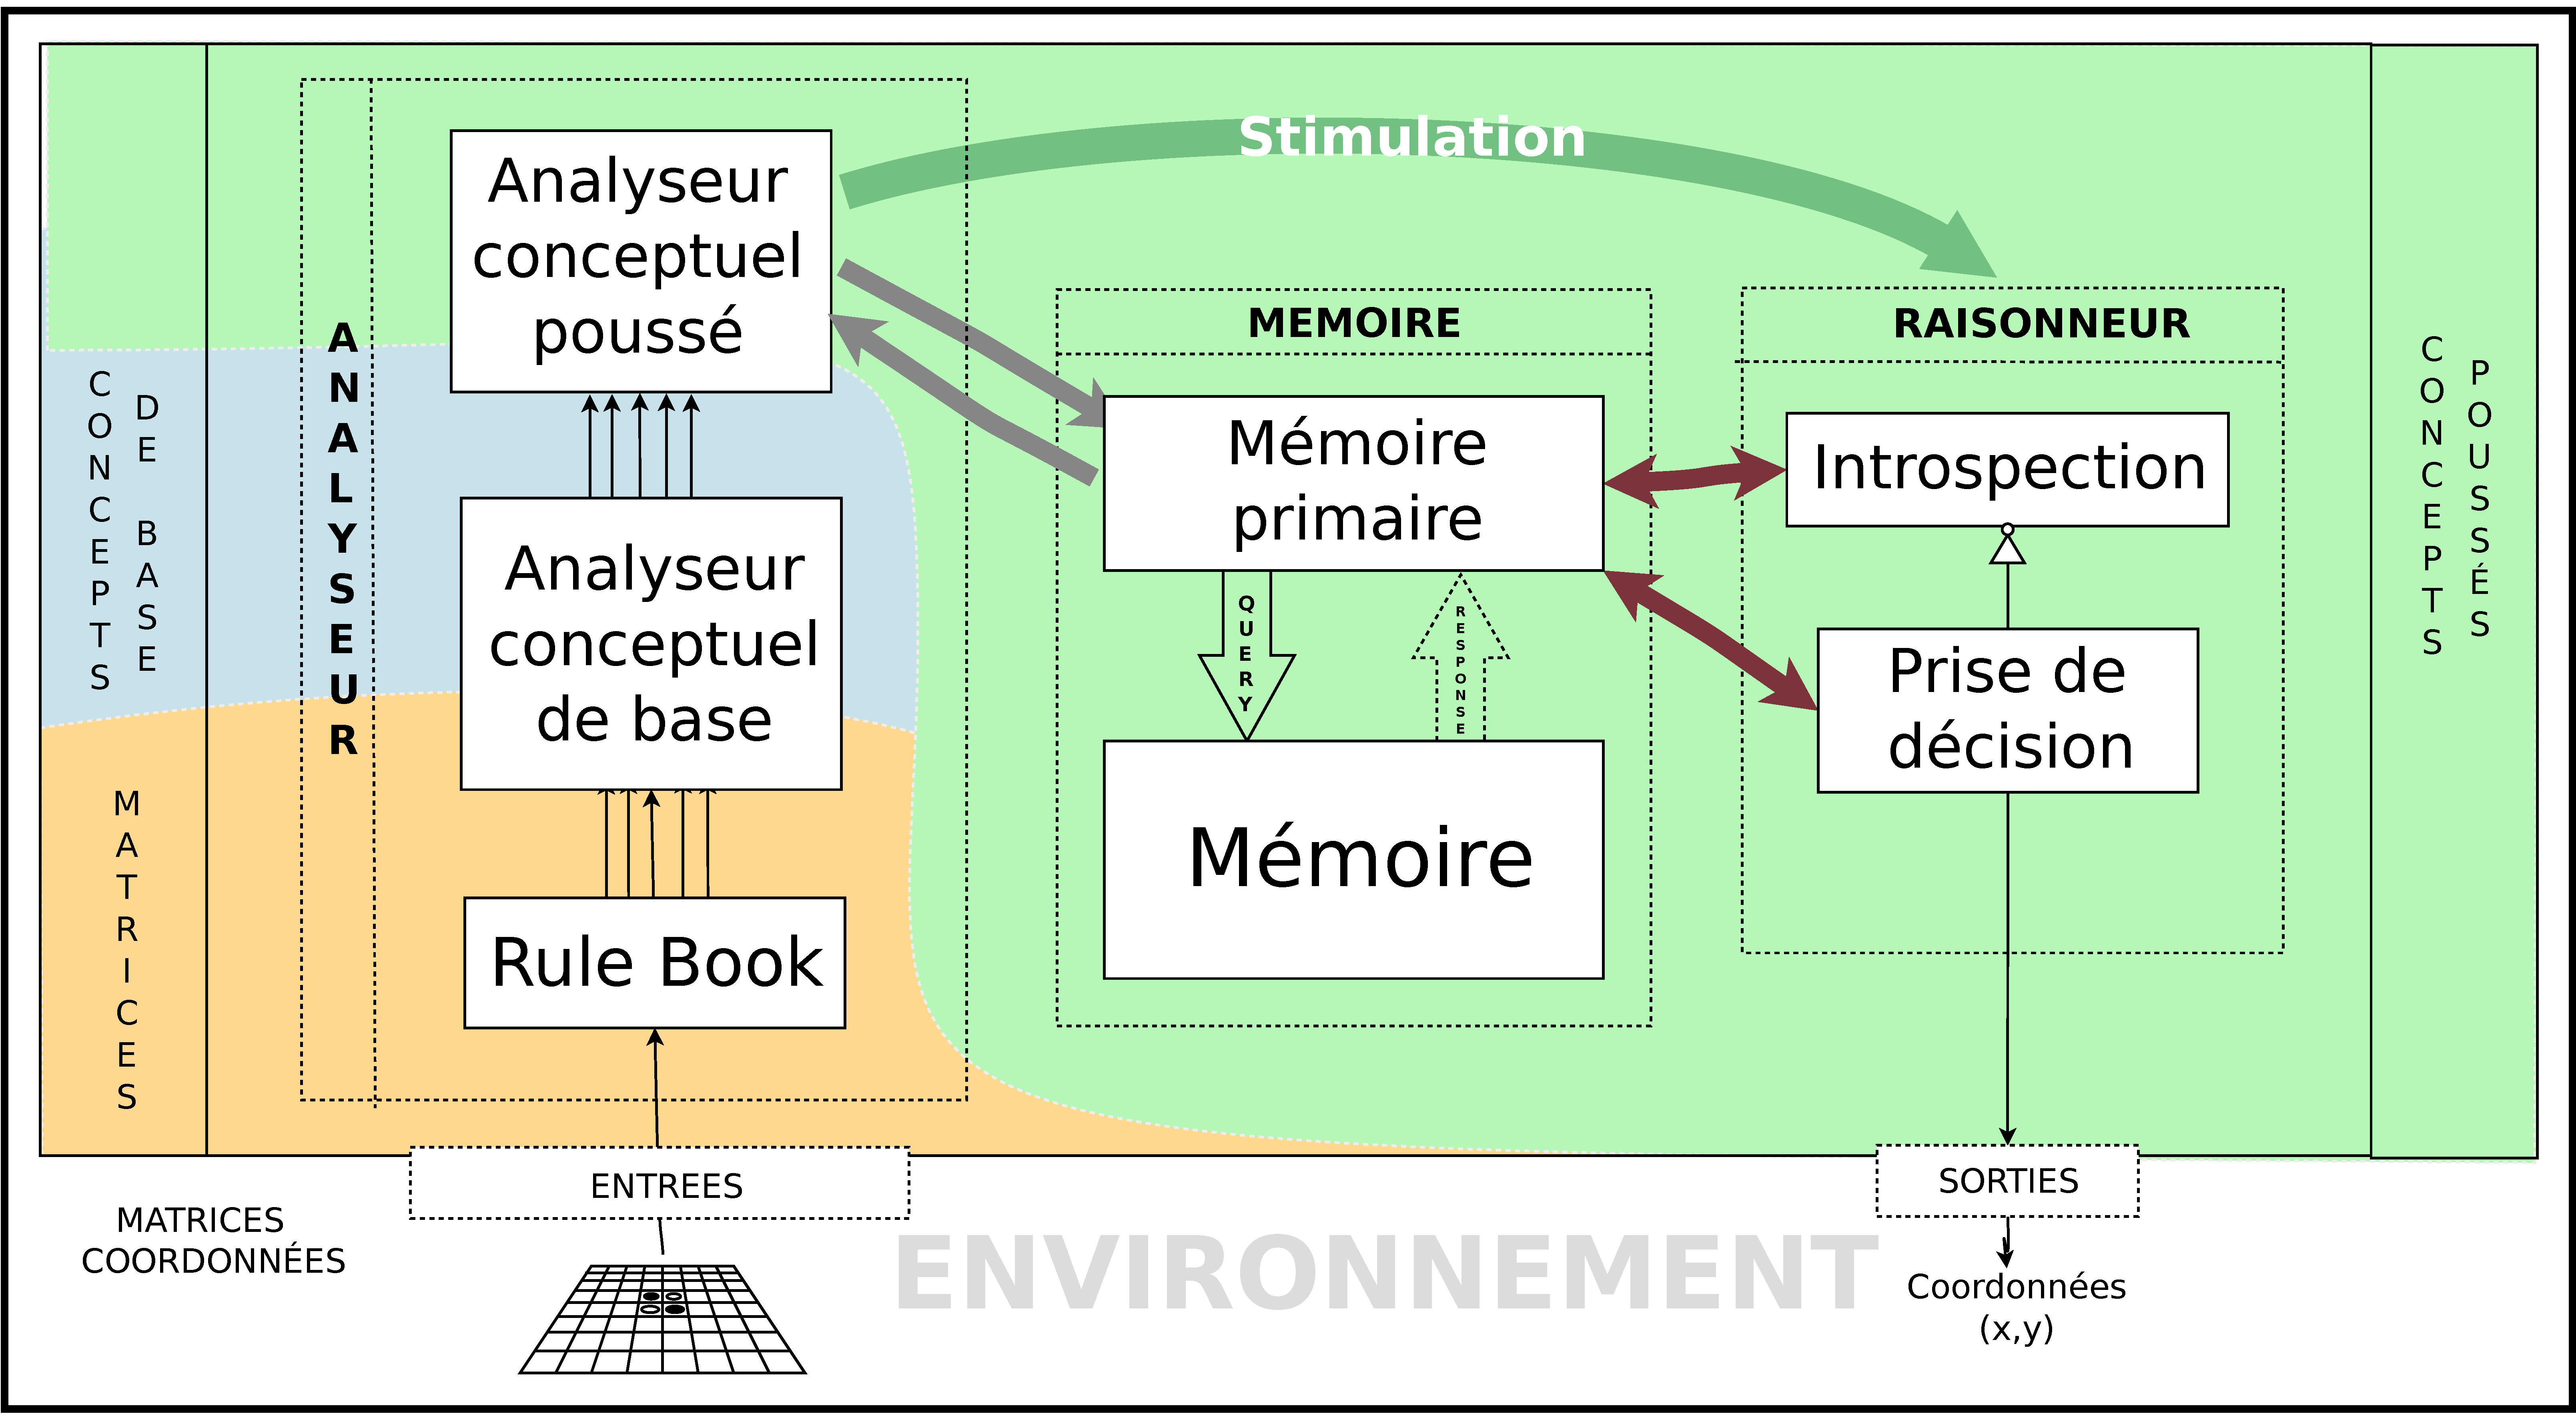
\includegraphics[width=\textwidth]{files/simplified_general_diagram} 
\caption{Schéma général} 
\label{schema_general}
\end{figure}
